%% Direttive TeXworks:
% !TeX root = ../semprini_luca_tesi.tex
% !TEX encoding = UTF-8 Unicode
% !TEX program = arara
% !TEX TS-program = arara
% !TeX spellcheck = it-IT

%% Direttive Arara:
% arara: pdflatex: { shell: yes, synctex: yes, action: batchmode, options: "-halt-on-error -file-line-error-style" }
% arara: frontespizio
% arara: biber
% arara: pdflatex: { shell: yes, synctex: yes, action: batchmode, options: "-halt-on-error -file-line-error-style" }
% arara: pdflatex: { shell: yes, synctex: yes, action: nonstopmode, options: "-halt-on-error -file-line-error-style" }
\chapter{Kotlin in Android}
Lo scopo primario dello sviluppo di Kotlin da parte di JetBrains non era, inizialmente, quello di trovare un nuovo linguaggio per sviluppare progetti Android. Tuttavia, appoggiandosi sulla JVM, fin dalla prima release sono state messe a fuoco le sue grandi potenzialità per costruire applicazioni su questa piattaforma. Con il passare dei mesi, questo contesto è divenuto il più popolare ed il più apprezzato dagli estimatori di Kotlin, tanto da portare, in via del tutto prematura e potenzialmente rischiosa, molte software house (ma anche sviluppatori indipendenti) a puntare su questo linguaggio per lo sviluppo delle proprie applicazioni mobile. Questa scommessa viene ripagata il 17 maggio 2017, data in cui il supporto ufficiale di Kotlin per questa piattaforma viene annunciato al Google I / O: da questa conferenza la popolarità del linguaggio di JetBrains cresce a dismisura ed il numero di progetti sviluppati interamente ed esclusivamente in Kotlin aumenta in maniera esponenziale.\\

\section{Perché Kotlin su Android?}
Il team di Android afferma di aver operato la scelta di rendere Kotlin un linguaggio ufficialmente supportato in quanto ritiene che sia "brillantemente progettato e maturo e renderà lo sviluppo di Android più veloce e divertente" \cite{ktOnAndroidDevBlog}; era già stato inoltre adottato, come accennato, da alcuni importanti sviluppatori (come Expedia, Flipboard, Pinterest, Square e altri) per le loro applicazioni di produzione. Un'altra discriminante nella scelta del supporto ufficiale è stata, ovviamente, "l'interoperabilità senza sforzo" con Java: i programmatori Android che utilizzano tradizionalmente Java non avranno alcune difficoltà nell’apprendere la sintassi e la filosofia di Kotlin e sarà per essi molto più semplice iniziare ad utilizzare sempre più il nuovo linguaggio di JetBrains nelle loro applicazioni. Inoltre, essendo un linguaggio sviluppato dalla medesima compagnia produttrice di IntelliJ IDEA (sulla quale, tra le altre cose, è basata la stessa IDE ufficiale di Google Android Studio), non sorprende che il supporto IDE per Kotlin sia certamente eccellente per un linguaggio così giovane: mentre nelle versioni precedenti dell'IDE, il supporto a Kotlin era garantito esclusivamente installando un opportuno plug-in, a partire da Android Studio 3.0, Kotlin diventa un linguaggio di programmazione totalmente supportato su Android \cite{ktUpdateAndroidDevBlog}, venendo completamente incorporato come linguaggio principale e lascia all'utente scegliere se compilare in un bytecode compatibile con Java 6 o con Java 8.\\

Le funzionalità linguistiche di Kotlin, combinate con un plug-in di compilazione che supporta il framework Android, possono trasformare lo sviluppo di applicazioni per questa piattaforma in un'esperienza molto più produttiva e piacevole. Pattern di programmazione molto comuni nello sviluppo, ad esempio l'aggiunta di \texttt{Listener} ai controlli o il binding degli elementi di layout ai campi, possono essere compiuti utilizzando molte meno linee di codice, o addirittura, a volte, senza bisogno di scrivere codice: il compilatore, infatti, può generare automaticamente parti consistenti di questi controlli. Un altro grande vantaggio di utilizzare Kotlin è la migliore affidabilità a livello di applicazione: spesso, infatti ci si imbatte in errori che portano al crash dell’intera applicazione, come un'eccezione non gestita (spesso, una \texttt{NullPointerException}); il sistema di tipi di Kotlin, con il suo preciso monitoraggio dei valori \texttt{null}, rende questo comune problema molto meno pressante. La maggior parte del codice che in Java avrebbe portato a una \texttt{NullPointerException}, non riesce a compilare in Kotlin, il che assicura di poter individuare l'errore a tempo di compilazione, quindi evitando crash inaspettati durante l’esecuzione. Allo stesso tempo, poiché Kotlin è completamente compatibile anche con Java 6, il suo utilizzo non introduce nessun tipo di preoccupazione a livello di compatibilità di codice. Un ulteriore vantaggio è rappresentato dall’utilizzo delle espressioni lambda: molte delle funzioni di standard library di Kotlin consentono di sintetizzarle in un’unica linea, rendendo il codice più compatto ed intuitivo.\\

\section{Funzionalità utili per lo sviluppo Android}
Sono state accennate nel paragrafo precedente alcune caratteristiche e pattern di programmazione incorporati da Kotlin che possono rendere lo sviluppo di applicazioni Android più intuitivo ed elegante. Di seguito saranno analizzati i più significativi.\\

\subsection{Lambda Expressions}
Le {\em Lambda Expressions}, o semplicemente lambda, sono essenzialmente frammenti di codice che possono essere passati ad altre funzioni e la loro introduzione in Java 8 è stato uno dei cambiamenti più attesi nell'evoluzione del principale linguaggio JVM. La standard library di Kotlin ne fa uso in maniera ampia e con esse è possibile estrarre facilmente strutture di codice comuni rendendole funzioni di libreria: le lambda possono essere utilizzate anche con le librerie Java, a conferma della piena interoperabilità tra i due linguaggi, anche con quelle che non sono state originariamente concepite per supportare espressioni lambda. Uno degli usi più comuni per questi particolari costrutti è utilizzarli per lavorare con le collezioni, o all'interno di listeners, nello specifico ambiente Android.\\

Passare e memorizzare pezzi di comportamento nel codice è un compito frequente quando si tratta di lavorare con progetti complessi: questo tipo di problema è affrontato principalmente dalla programmazione funzionale, che offre un approccio differente da quello della programmazione Object-Oriented per risolvere questa questione; essa offre, infatti, la capacità di trattare le funzioni come valori. Invece di dichiarare una classe e di passarne un'istanza ad un metodo, è possibile passare direttamente una funzione, rendendo il codice è ancora più conciso. Non è necessario, inoltre, dichiarare esplicitamente una funzione, ma si può decidere di passare un blocco di codice direttamente come parametro di metodo. Di seguito si riporta nell'esempio \ref{lst:exAmpleLambda} una definizione di un Listener responsabile della gestione di click in Java 7. Questo ascoltatore implementa la corrispondente interfaccia \texttt{OnClickListener} con un metodo, \texttt{onClick}:\\

\begin{lstlisting}[caption={Definizione di \texttt{OnClickListener} in Java}, captionpos=b, label={lst:exAmpleLambda}, language=Java]
button.setOnClickListener(new OnClickListener() {
  @Override
  public void onClick(View view) {
      /* actions on click */
  }
});
\end{lstlisting}

Si noti la verbosità eccessiva, necessaria per dichiarare una classe interna anonima per esprimere il comportamento di un bottone nel momento in cui viene cliccato: questo pattern, se ripetuto molte volte, aumenta la complessità e intacca la leggibilità di un programma. In Kotlin, come in Java 8, è possibile utilizzare una lambda per questo comportamento:\\

\begin{lstlisting}[caption={Definizione di una lambda in Kotlin}, captionpos=b, label={lst:exAmpleLambdaConciso}, language=Kotlin]
button.setOnClickListener { view -> /* ... actions on click */ }
\end{lstlisting}

Lo snippet di codice nell'esempio \ref{lst:exAmpleLambdaConciso} Kotlin opera allo stesso modo di una classe anonima in Java (come nell'esempio \ref{lst:exAmpleLambda}) ma risulta molto più conciso e leggibile.\\
Un classico uso delle espressioni lambda è effettuato nel contesto delle Collezioni: la maggior parte delle attività che coinvolgono il Collection framework, infatti, seguono alcuni pattern comuni, quindi il codice che li implementa dovrebbe essere standardizzato in una qualche libreria; tuttavia questo risulta difficile senza fare uso di lambda.\\
Un classico esempio di come Kotlin integra all'interno della sua standard library delle funzioni che permettono, attraverso l'uso delle lambda, di semplificare il lavoro con le collezioni è la funzione \texttt{maxBy}, che permette di trovare il massimo elemento di una qualsiasi collezione, specificando quali valori debbano essere confrontati per trovarlo, appunto attraverso una lambda expression:\\

\begin{lstlisting}[caption={La funzione \texttt{maxBy}}, captionpos=b, label={lst:exAmpleLambdamaxBy}, language=Kotlin]
val people = listOf(Person("Frank", 29), Person("Bob", 31))
people.maxBy({ p: Person -> p.age })  // Stampa "Person(name=Bob, age=31)"
\end{lstlisting}

Nell'esempio \ref{lst:exAmpleLambdamaxBy} si suppone di aver definito una semplice classe \texttt{Person}, che prenda come parametri il nome di battesimo e l'età di una persona, quindi leggermente differente da quella definita nel capitolo precedente. La funzione \texttt{maxBy}, in questo specifico caso, è chiamata per trovare la persona più anziana all’interno della lista \texttt{people}, senza fare uso esplicito di cicli: il codice tra le parentesi graffe \texttt{{ p: Person -> p.age }} è una lambda che attua questa specifica logica. La funzione riceve un oggetto \texttt{Person} della lista come argomento (referenziato dalla variabile "\texttt{p}") e restituisce un valore da confrontare, in questo caso specifico si tratta dell'età, immagazzinata nella proprietà "\texttt{age}". Tuttavia questo codice risulta ancora alquanto verboso: in primo luogo, vi è ancora troppa punteggiatura, che danneggia la leggibilità, inoltre il tipo \texttt{Person} può essere dedotto dal contesto da parte del compilatore e quindi può essere omesso; infine, in Kotlin, non è necessario assegnare un nome all'argomento che prende in ingresso la lambda in questo caso.\\
Di seguito, verranno forniti esempi in cui si eseguiranno miglioramenti graduali alla sintassi, fino ad arrivare ad una forma espressiva ideale e che rispetti appieno la filosofia di Kotlin. Come prima cosa si rimuoveranno le parentesi: una convenzione sintattica consente di spostare una espressione lambda dalle parentesi tonde se essa è l'ultimo argomento in una chiamata di funzione. In questo esempio specifico (\ref{lst:exAmpleLambdamaxByNoPar}), tuttavia, la lambda expression è l'unico argomento, quindi è anche possibile rimuovere completamente le parentesi tonde dalla chiamata:\\

\begin{lstlisting}[caption={Rimozione delle parentesi tonde}, captionpos=b, label={lst:exAmpleLambdamaxByNoPar}, language=Kotlin]
people.maxBy { p: Person -> p.age }
\end{lstlisting}

Queste differenti forme sintattiche hanno esattamente la stessa semantica, con la differenza che l'ultima risulta essere la più semplice da leggere. Nel caso in cui si voglia passare due o più lambda, non è possibile muoverne più di una, quindi è tipicamente consigliabile passarle utilizzando la sintassi regolare.\\
Procedendo con la semplificazione della sintassi, come accennato precedentemente, si può facilmente notare che si può fare a meno di specificare il tipo del parametro che la lambda prende in ingresso, in quanto il compilatore di Kotlin riuscirà a dedurlo dal contesto:\\

\begin{lstlisting}[caption={Rimozione della specificazione di tipo dalla lambda}, captionpos=b, label={lst:exAmpleLambdamaxByNoType}, language=Kotlin]
people.maxBy { p -> p.age }
\end{lstlisting}

Con la funzione \texttt{maxBy}, in particolare, il tipo del parametro è sempre uguale al tipo dell'elemento della collezione: siccome in questo caso si sta chiamando \texttt{maxBy} su una collection di oggetti \texttt{Person}, il compilatore riesce ad inferire che anche il parametro "\texttt{p}" sarà di tipo \texttt{Person}.\\
L'ultima semplificazione che si può fare su questo esempio è la sostituzione dell'argomento con il nome di argomento predefinito: \texttt{it}. Questo nome viene generato se il contesto prevede una lambda con un solo argomento, e il suo tipo può essere dedotto:\\

\begin{lstlisting}[caption={Utilizzo della kewyword "it" all'interno della lambda}, captionpos=b, label={lst:exAmpleLambdamaxByIt}, language=Kotlin]
people.maxBy { it.age }
\end{lstlisting}

"\texttt{it}" è un nome di argomento auto-generato e si tratta di una convenzione ottima per abbreviare il codice, ma non va abusata. In particolare, nel caso di lambda innestate, è consigliabile dichiarare esplicitamente il parametro di ciascuna lambda, per evitare di non riuscire a capire a quale valore si fa riferimento all'interno del codice; inoltre dichiarare i parametri esplicitamente risulta necessario anche se il significato o il tipo del parametro non è deducibile dal contesto (ad esempio quando si memorizza una lambda all'interno di una variabile). In tutti gli altri casi è utile utilizzare la keyword \texttt{it} per aggiungere un ulteriore livello di espressività e concisione.\\
Tuttavia, in Kotlin, se una lambda fa semplicemente riferimento a un metodo o una proprietà, esiste un'ulteriore forma espressiva; può anche essere sostituita, infatti, da una cosiddetta "{\em member reference}", con la seguente sintassi:\\

\begin{lstlisting}[caption={Member reference}, captionpos=b, label={lst:exAmpleLambdaMember}, language=Kotlin]
println(people.maxBy(Person::age))
\end{lstlisting}

Per quanto riguarda nello specifico il contesto Android, c'è da dire che la maggior parte delle API con cui è necessario lavorare per costruire un'applicazione sono scritte in Java; questo tuttavia non rappresenta un problema, in quanto le lambda di Kotlin sono completamente interoperabili con le API Java. Nell'esempio \ref{lst:exAmpleLambdaConciso} presentato all'inizio del paragrafo, si è utilizzata una lambda Kotlin per implementare il metodo \texttt{onClick} di un \texttt{OnClickListener} Java (che ha un solo parametro di tipo \texttt{View} come anche lo stesso metodo \texttt{onClick}).  Ciò è possibile poiché \texttt{OnClickListener} ha solo un metodo astratto: questi particolari tipi di interfacce sono chiamate {\bfseries interfacce funzionali,} o {\bfseries interfacce SAM} (Single Abstract Method). Le API Java forniscono una vasta gamma di interfacce funzionali come \texttt{Runnable} e \texttt{Callable}, così come i metodi che lavorano con esse: Kotlin permette di usare lambda expressions quando si chiamano metodi Java che prendono interfacce funzionali come parametri, facendo in modo che il codice Kotlin rimanga pulito e idiomatico.\\
In conclusione, è possibile passare una lambda a qualsiasi metodo Java che preveda un'interfaccia funzionale; in aggiunta, si avranno a disposizione tutte le forme espressive delle lambda Kotlin di cui si è discusso in precedenza, permettendo una potenza semantica nel chiamare metodi che prevedano in ingresso un'interfaccia funzionale (come, ad esempio, gli stessi \texttt{setOnClickListener}, di cui si fa largo uso nei progetti Android) che in Java non sarebbe presente:\\
\\

\begin{lstlisting}[caption={Definizione di OnClickListener con le varie forme espressive di Kotlin}, captionpos=b, label={lst:exAmpleLambdaList}, language=Kotlin]
view.setOnClickListener( { v: View -> doSomething(v) } )  // Costrutto verboso
view.setOnClickListener() { v: View -> doSomething(v) }   // Costrutto con parentesi tonde
view.setOnClickListener { v -> doSomething(v) }           // Rimozione di parentesi e tipo
view.setOnClickListener { doSomething(it) }               //Costrutto pulito utilizzando "it"
\end{lstlisting}

\subsection{Operator Overloading}
La capacità di definire funzioni che, quando chiamate, permettono di utilizzare gli operatori è chiamata
{\bfseries Operator Overloading}. In generale, le filosofie dei diversi linguaggi di programmazione possono consentire nell'utilizzare questo tipo di approccio in maniera molto limitata (come accade nel caso specifico di Java, in cui l'insieme delle cosiddette {\em operator functions} è fissato e ristretto e non è permesso allo sviluppatore di crearne ad hoc), oppure essere molto più permissive, come nel caso di Scala. I progettisti di Kotlin hanno optato per una filosofia che si collocasse da qualche parte nel mezzo di questi estremi, consentendo al programmatore di effettuare operator overloading in maniera fissa e controllata. Vi è, infatti, un elenco fissato (seppur molto ampio) di operatori che possono essere usati come funzioni, ma tutte le combinazioni arbitrarie sono proibite. Per creare una tale funzione, essa deve essere preceduta, in fase di dichiarazione, dalla parola chiave "\texttt{operator}" e definita usando l'equivalente inglese del nome dell'operatore: in Kotlin, infatti, tutti gli operatori hanno un nome equivalente inglese predefinito che viene utilizzato per fare overloading sugli stessi, quindi, per esempio, la funzione "\texttt{sum}" permetterà di fare overloading dell'operatore "\texttt{+}", la funzione "\texttt{minus}" dell'operatore {\texttt{-}}, la funzione \texttt{equals} dell'operatore \texttt{==}, e così via. Ciò che accade a livello di compilazione in questo caso è una semplice sostituzione dell'operatore con una invocazione della operator function corrispondente.\\
Una similitudine in Java può essere rappresentata dalla possibilità di utilizzare, ad esempio, gli oggetti che implementano \texttt{java.lang.Iterable} all'interno dei for-loop e gli oggetti che implementano \texttt{java.lang.AutoCloseable} all'interno di statement {\em try-with-resources}. L'operator overloading di Kotlin risulta in confronto molto più potente, in quanto, invece di essere legate a specifici tipi, tali funzionalità sono legate, appunto, a funzioni con nomi specifici. Quando ci si riferisce a questa funzionalità si parla di una vera e propria {\em convenzione}. Invece di fare affidamento sui tipi come in Java, questo consente a Kotlin di adattare le classi Java esistenti ai requisiti delle caratteristiche linguistiche di Kotlin: l'insieme delle interfacce implementate da una classe di libreria Java è fisso e non è possibile modificarla in modo da aggiungerne ulteriori. D'altra parte, la definizione di nuovi metodi per una classe è possibile grazie al meccanismo delle extension functions. In Kotlin, dunque, tutti i metodi convenzionali di operator overloading vengono definiti come estensioni, consentendo quindi di adattare qualsiasi classe Java esistente senza modificarne il codice. Questa operazione è consentita su diverse famiglie di operatori.\\

\subsubsection{Operatori Aritmetici}
L'esempio più semplice dell'uso delle convenzioni di operator overloading in Kotlin sono gli operatori aritmetici. In Java, il set completo di operazioni aritmetiche può essere utilizzato solo con i tipi primitivi e, nel caso di eccezione dell'operatore "\texttt{+}" con i valori \texttt{String}; in Kotlin l'uso queste operazioni viene consentito in maniera molto più ampia: ad esempio, se si sta utilizzando la classe \texttt{BigInteger} risulta più elegante da sommare due istanze di questa classe utilizzando direttamente l'operatore "\texttt{+}", invece di chiamare esplicitamente il metodo di aggiunta; oppure, per aggiungere un elemento a una collezione, si consiglia di utilizzare l'operatore "\texttt{+=}". Esistono moltissime applicazioni di operator overloading su operatori aritmetici, di seguito viene riportato, nell'esempio \ref{lst:exAmpleOpOv}, l'overloading di un operatore aritmetico binario nello specifico campo Android:\\

\begin{lstlisting}[caption={Operatore aritmeticos su una lista}, captionpos=b, label={lst:exAmpleOpOv}, language=Kotlin]
val emptyButton = Button(this)	        //Creazione di un "dummy" Button
val listOfButtons = ArrayList<Button>() //Lista vuota di Button
listOfButtons += emptyButton            //Aggiunta di emptyButton nella lista
\end{lstlisting}

\subsubsection{Operatori di Confronto}
Proprio come con gli operatori aritmetici, Kotlin consente di utilizzare gli operatori di confronto (\texttt{==}, \texttt{!=}, \texttt{>}, \texttt{<}, ecc.) con qualsiasi oggetto, non solo con i tipi primitivi. Invece di chiamare metodi come \texttt{equals} oppure \texttt{compareTo}, è possibile utilizzare (potenzialmente su qualsiasi oggetto) direttamente gli operatori di confronto, rendendo il codice più intuitivo e conciso.\\

\subsubsection{Operatori di Collezioni e Range}
Alcune delle operazioni più comuni utilizzate nel lavorare con le collezioni possono essere quelle di getting e setting di un elemento specificandone l'indice, o verificare se un elemento appartiene a una Collection. Questo tipo di operazioni sono supportate tramite la sintassi dell'operator overloading nella libreria standard di Kotlin: per ottenere o settare un elemento per indice, si può utilizzare la sintassi \texttt{a[b]} (chiamata "{\em index operator}"); mentre l'operatore "\texttt{in}" può essere utilizzato per controllare se un elemento è presente in una Collection o in un range di valori, ma anche per iterare su una collezione. Il fatto di poter aggiungere queste operazioni per le proprie classi che agiscono come collezioni, può risultare un aiuto molto utile in Android: in particolare, all'interno di un \texttt{Adapter} per una \texttt{RecyclerView} o in blocchi di codice che utilizzano dei \texttt{ViewGroup} può risultare molto più elegante fare uso di index operator nei seguenti modi:\\

\begin{lstlisting}[caption={Operator Overloading su \texttt{ViewGroup}}, captionpos=b, label={lst:exAmpleOpOvViewGroup}, language=Kotlin]
val views = //...
val first = views[0]
views -= first
views += first
if (first in views) doSomething()

/*  Definizione degli operatori  */

operator fun ViewGroup.get(index: Int): View? = getChildAt(index)
operator fun ViewGroup.minusAssign(child: View) = removeView(child)
operator fun ViewGroup.plusAssign(child: View) = addView(child)
operator fun ViewGroup.contains(child: View) = indexOfChild(child) != -1
\end{lstlisting}

Si supponga ora di aver creato una classe che faccia da wrapper per una lista, ad esempio, di oggetti \texttt{Person}, per cui si vuole avere delle informazioni aggiuntive, come la città e il Paese relativi alla specifica lista di persone; supponendo di voler utilizzare questa lista per riempire una \texttt{RecyclerView}, può essere utile aggiungere i seguenti metodi:\\

\begin{lstlisting}[caption={Definizione di operator functions per una \texttt{PersonList}}, captionpos=b, label={lst:exAmpleOpOvRecView}, language=Kotlin]
data class PersonList(val city: String, val country: String, val list : List<Person>) {
  val size: Int get() = list.size
  operator fun get(position: Int) = list[position]
}
\end{lstlisting}

Ora, all'interno dei metodi \texttt{onBindViewHolder} e \texttt{getItemCount} dell'\texttt{Adapter} di questa ipotetica \texttt{RecyclerView}, sarà possibile semplificare alcune chiamate, come si può notare nell'esempio \ref{lst:exAmpleOpOvRecViewAdapter}:\\

\begin{lstlisting}[caption={Utilizzo degli operatori in un \texttt{Adapter}}, captionpos=b, label={lst:exAmpleOpOvRecViewAdapter}, language=Kotlin]
class PersonListAdapter(private val myList: PersonList) {

  /* ... */

  override fun onBindViewHolder(holder: ViewHolder, position: Int) {
      	with(myList[position]) {
	         holder.textView.text = "Name: $name, Age: $age"
        }
  }
  override fun getItemCount() = myList.size

  /* ... */
}
\end{lstlisting}

\subsection{Annotazioni}
Le annotazioni sono mezzi per associare dei metadati al proprio codice, tipicamente alla dichiarazione di una classe o metodo; la sintassi per l'utilizzo di questo espediente è esattamente uguale a quella che si usa in Java, mentre per quanto riguarda la dichiarazione delle proprie classi di annotazione è leggermente differente. La maggior parte dei framework Java moderni utilizza ampiamente le annotazioni, quindi non è un concetto introdotto ex novo dal linguaggio Kotlin, ma vi sono alcune funzionalità aggiuntive e interessanti soprattutto nell'ambito della programmazione Android.\\
Come accennato, la sintassi è la stessa di Java: per applicare un'annotazione, si inserisce il suo nome, preceduto dal carattere "\texttt{@}", all'inizio della dichiarazione che si sta annotando. Ad esempio, se si utilizza il framework JUnit, è possibile contrassegnare un metodo di prova con l'annotazione \texttt{@Test}:\\

\begin{lstlisting}[caption={Annotazione di Test}, captionpos=b, label={lst:exAmpleAnnotTest}, language=Kotlin]
import org.junit.*

class MyTest {
  @Test fun testTrue() {
    Assert.assertTrue(true)
  }
}
\end{lstlisting}
L'annotazione \texttt{@Test}, come in Java, comunica al framework JUnit di invocare il metodo \texttt{testTrue()} come test.\\

Un esempio decisamente più interessante, in ambito Android, è rappresentato dall'annotazione \texttt{@Deprecated}: il suo significato in Kotlin è lo stesso di Java, tuttavia viene perfezionata e resa più specifica, introducendo il parametro \texttt{replaceWith}, che consente di fornire un pattern di sostituzione per supportare una transizione più guidata ad una nuova versione dell'API. Nell'esempio \ref{lst:exAmpleAnnotDepr} viene illustrato come è possibile fornire argomenti per questa specifica annotazione, un messaggio di deprecazione e un pattern di sostituzione:\\

\begin{lstlisting}[caption={Utilizzo dell'annotazione \texttt{@Deprecated}}, captionpos=b, label={lst:exAmpleAnnotDepr}, language=Kotlin]
@Deprecated(level = DeprecationLevel.ERROR,
        	  message = "Use class StringUtils instead!", /* Il mio messaggio */
        	  replaceWith = ReplaceWith(
                expression = "StringUtils.isEmpty(input)",
                imports = {"org.apache.commons.lang3.StringUtils"}))
public static boolean isEmpty(String input) {
    return input.equals("");    /* Metodo Java */
}
\end{lstlisting}

Gli argomenti dell'annotazione vengono passati tra parentesi, proprio come in una normale chiamata di funzione: come si può notare, \texttt{@Deprecated} prende in ingresso, oltre al messaggio custom che si vuole mostrare, un oggetto di tipo \texttt{ReplaceWith}, che a sua volta accetta due parametri: "\texttt{expression}", che rappresenta la funzione da utilizzare in sostituzione di quella che si sta dichiarando come deprecata, ed "\texttt{imports}", che specifica gli eventuali import da eseguire per trovare la funzione di sostituzione. \texttt{@Deprecated} accetta un altro parametro di input, che è facoltativo e rappresenta il "livello" di deprecazione: nell'esempio \ref{lst:exAmpleAnnotDepr}, siccome è specificato il livello \texttt{ERROR}, quando si andrà a chiamare la funzione deprecata \texttt{isEmpty}, il compilatore segnalerà la chiamata come {\bfseries errore} (non permetterà, quindi, di compilare il codice) finché non la si andrà a sostituire con la funzione adeguata (specificata dal parametro di tipo \texttt{ReplaceWith}). Con questa dichiarazione, se qualche metodo utilizza la funzione \texttt{isEmpty} definita nell’esempio, l'IDE su cui si sta lavorando non solo mostrerà quale funzione deve essere utilizzata al posto di questa \texttt{isEmpty} deprecata (la funzione \texttt{isEmpty} della classe \texttt{StringUtils}, nell'esempio \ref{lst:exAmpleAnnotDepr}), ma offrirà anche una soluzione rapida per sostituirla automaticamente (tipicamente con la combinazione di tasti \texttt{Alt+Invio}, in IntelliJ ed AndroidStudio).\\

\begin{figure}[ht]
  \centering
  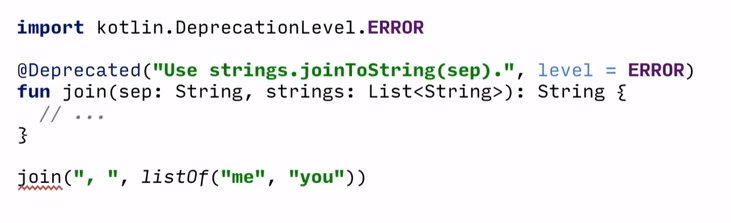
\includegraphics[scale=0.75]{DeprecationLevel.png}
  \caption{{\bfseries Errore a compile-time con \texttt{DeprecationLevel.ERROR}}}
  \label{deprecationError}
\end{figure}

\begin{figure}[ht]
  \centering
  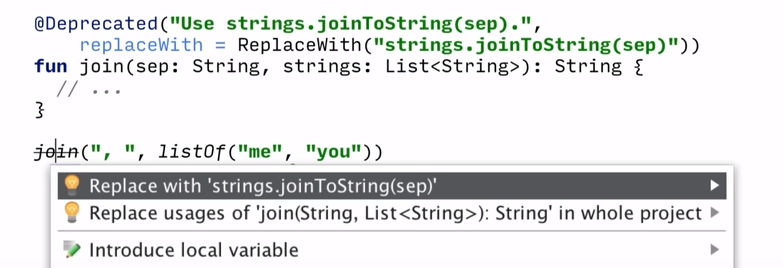
\includegraphics[scale=0.75]{DeprecationReplaceWith.png}
  \caption{{\bfseries Sostituzione a livello di IDE grazie al parametro \texttt{ReplaceWith}}}
  \label{deprecationWarning}
\end{figure}


Le annotazioni possono accettare come parametri soltanto tipi primitivi, stringhe, enumerazioni, riferimenti di classe, e array. La sintassi per specificare argomenti di annotazioni è leggermente diversa da Java.\\
Per specificare una classe come argomento di annotazione, è necessario inserire "\texttt{::class}" dopo il nome della classe, in questo modo:\\

\begin{lstlisting}[caption={Definizione di una annotazione personalizzata}, captionpos=b, label={lst:exAmpleAnnotCust}, language=Kotlin]
@MyAnnotation(MyClass::class)
\end{lstlisting}

Gli argomenti di annotazione devono essere noti al momento della compilazione, quindi se si intende utilizzare una proprietà come argomento di annotazione, è necessario contrassegnarla con il modificatore "\texttt{const}" (quindi deve essere inizializzata con valori di tipi primitivi o \texttt{String}), che riferisce al compilatore che la proprietà è una costante a compile-time.\\

\subsection{Coroutines}
Alcune API si servono di operazioni di tipo long-running (ad esempio operazioni di network IO, file IO, lavori intensivi su CPU o GPU, ecc.) e richiedono che il chiamante blocchi la propria esecuzione fino a quando esse non giungono al termine. Le {\em Kotlin Coroutines} forniscono un modo per evitare di eseguire manualmente blocchi sui thread e sostituire questa pratica con un'operazione più economica e controllabile: la sospensione di una coroutine.\\
Esse, infatti, semplificano la programmazione asincrona inserendo la logica della compilazione thread-safe nelle librerie: la logica del programma può essere espressa sequenzialmente in una coroutine, e la libreria sottostante intuirà l'asincronia in maniera trasparente. La libreria può wrappare parti rilevanti del codice utente in callback, sottoscrivere eventi rilevanti, schedulare l'esecuzione su thread diversi (o anche macchine diverse), lasciando che il codice rimanga semplice ed intuitivo come se fosse eseguito in sequenza. La sospensione di Coroutine è quasi gratuita: non è necessario alcun switch di contesto o qualsiasi altro coinvolgimento del sistema operativo. Molti meccanismi asincroni disponibili in altri linguaggi possono essere implementati ad hoc come librerie usando le coroutines di Kotlin: per fare alcuni esempi, si parla delle {\em async/await} di C\# \cite{asyawaitCSh} e JavaScript, {\em channels} e {\em select} da Go, e {\em generator/yield} da C\# e Python \cite{generatorPY}.\\
Le Coroutines sono state la più grande novità nella release Kotlin v1.1 ed hanno suscitato molto entusiasmo all'interno della community a causa delle loro potenzialità. Tuttavia, sono un meccanismo ancora in fase sperimentale, che avrà la sua versione stabile solo con Kotlin v1.2 \cite{kotlinV11}.\\
Riassumendo, le coroutines si basano sull'idea di sospendere certe funzioni: quelle che possono bloccare l'esecuzione del programma nel momento in cui vengono chiamate e farla proseguire dopo aver terminato l'esecuzione del proprio compito: queste cosiddette "{\em suspending functions}" o funzioni di sospensione sono contrassegnate dalla parola chiave \texttt{suspend} e possono accettare parametri di ingresso e restituire valori in uscita allo stesso modo delle normali funzioni, ma possono essere chiamate solo all'interno di altre funzioni di sospensione o all'interno di una coroutine (d'altra parte, la libreria può decidere di procedere senza sospensione se il risultato della chiamata in questione è già disponibile); ciò significa che non è possibile invocarle in qualunque parte all'interno del codice, ma deve esserci una funzione circostante che costruisca la coroutine e fornisca il contesto richiesto per farlo. Una funzione di sospensione viene dichiarata con la seguente sintassi:\\

\begin{lstlisting}[caption={Definizione di una funzione di sospensione}, captionpos=b, label={lst:exAmpleSusp}, language=Kotlin]
suspend fun mySuspendingFunction(someParam: Int): Boolean {
    /* ... */
}
\end{lstlisting}

Un esempio semplificato di funzione \texttt{async} (disponibile nelle libreria \texttt{kotlinx.coroutines}) che permetta di fare chiamate a funzioni di sospensione è il \ref{lst:exAmpleAsync}:\\

\begin{lstlisting}[caption={Semplificazione della definizione della funzione di libreria \texttt{async}}, captionpos=b, label={lst:exAmpleAsync}, language=Kotlin]
fun <T> async(block: suspend () -> T)
\end{lstlisting}

Come si può notare, nell'esempio \ref{lst:exAmpleAsync}, \texttt{async} è una normale funzione (non di sospensione), ma il parametro "\texttt{block}" ha un function type con il modifier \texttt{suspend}: questo significa che quando viene passata un lambda a questa funzione, si tratterà di una lambda di sospensione, che permetterà di chiamare una funzione di sospensione al suo interno, nel seguente modo:\\

\begin{lstlisting}[caption={Utilizzo della funzione \texttt{async}}, captionpos=b, label={lst:exAmpleAsyncCall}, language=Kotlin]
async {
    mySuspendingFunction(someParam)

    /*...*/
}
\end{lstlisting}

Per arricchire l'esempio, la funzione \texttt{await} può essere una funzione di sospensione (quindi invocabile da un blocco \texttt{async{}}) che sospende una coroutine fino a quando non viene eseguito un certo tipo di computazione e restituisce il risultato:\\

\begin{lstlisting}[caption={Combinazione \texttt{async / await}}, captionpos=b, label={lst:exAmpleAwait}, language=Kotlin]
async {
    val resultOfAwait = computation.await()

    /*...*/
}
\end{lstlisting}

Discutendo del funzionamento interno, le coroutines sono interamente implementate attraverso una tecnica di compilazione (non è richiesto alcun supporto dal lato VM o OS) e la sospensione funziona tramite la trasformazione di codice. Fondamentalmente, ogni funzione di sospensione viene trasformata in una State Machine dove gli stati corrispondono alle chiamate di sospensione. Appena prima di una sospensione, lo stato successivo viene memorizzato in un campo di una classe generata dal compilatore insieme a variabili locali rilevanti e, una volta ripresa quella coroutine, le variabili locali vengono ripristinate e la macchina a stati procede dallo stato immediatamente successivo alla sospensione. Una coroutine sospesa può essere memorizzata e passata come un oggetto che mantiene lo stato di sospensione e le variabili locali. Il tipo assegnato a tali oggetti è \texttt{Continuation} e la trasformazione complessiva del codice citata corrisponde allo stile {\em Continuation-passing} proprio della programmazione funzionale. Di conseguenza, le funzioni di sospensione accettano in ingresso un ulteriore parametro di tipo \texttt{Continuation} in modo trasparente.\\

Nel contesto Android, le coroutine risultano molto utili, in quanto ci si può trovare molto facilmente ad utilizzare del codice asincrono, soprattutto lavorando con la GUI. Un esempio pragmatico di utilizzo di coroutines può essere rappresentato dal caricamento asincrono di due immagini (magari pesanti) all'interno di due differenti \texttt{View}:\\

\begin{lstlisting}[caption={Utilizzo di funzioni di libreria per Coroutines in Android}, captionpos=b, label={lst:exAmpleAsyncView}, language=Kotlin]
val first = loadImageAsync("green")
val second = loadImageAsync("red")
overlay(first.await(), second.await())
fun loadImageAsync(name: String) = async { /* ... */ }
\end{lstlisting}

La popolare libreria Anko, di cui si discuterà in seguito, fornisce molte soluzioni per implementare coroutines in maniera efficiente ed intuitiva in ambiente Android.\\

\section{Librerie}
Nonostante il linguaggio Kotlin si presti particolarmente a portare maggior fluidità e concisione nella programmazione di applicazioni Android, esistono diverse librerie che permettono di semplificare in maniera ancora superiore certe fasi dello sviluppo e certe caratteristiche dell'applicazione. Alcune di queste sono state sviluppate prima ancora che Kotlin ottenesse il titolo di linguaggio ufficialmente supportato da Google, quindi, una volta avvenuto l'annuncio al Google I / O 2017 \cite{googleio}, hanno subito, insieme al linguaggio stesso una considerevole impennata nell'utilizzo da parte degli sviluppatori\\
Di seguito verranno menzionate le librerie più popolari e significative per lo sviluppo di sistemi Android; tuttavia, si consideri il fatto che, essendo Kotlin un linguaggio molto giovane ed ufficializzato da poco per la programmazione Android, queste ultime sono in continua e inesorabile espansione, pertanto verranno sicuramente ampliate e migliorate nel corso dei prossimi mesi e anni.\\

\subsection{Kotlin Android Extensions}
Questa libreria (a cui ci si riferisce anche con l’acronimo {\bfseries KAE}) non è più considerata tale circa dall'avvento di Kotlin v1.0, in quanto integrata automaticamente all'interno delle dipendenze Gradle per la compilazione di progetti Kotlin. Si tratta di una valida ed economica alternativa alla popolare Butter Knife (scritta in Java ed utilizzata soprattutto per effettuare view-binding semplificato): essendo un plugin integrato nel compilatore Kotlin non richiede aggiuntivo overhead a runtime.\\
L'import all'interno di un file Kotlin viene effettuato tipicamente in maniera automatica da Android Studio, aggiungendo le linee di codice definite nell'esempio \ref{lst:exAmpleImportKAE}:\\

\begin{lstlisting}[caption={Import delle Kotlin Android Extensions}, captionpos=b, label={lst:exAmpleImportKAE}, language=Kotlin]
import kotlinx.android.synthetic.main.<layout>.*      //Oppure
import kotlinx.android.synthetic.main.<layout>.view.*
\end{lstlisting}

L'utilizzo di queste Extensions risulta molto intuitivo ed immediato. Si parla di proprietà {\em synthetic} quando ci si riferisce a quella parte della libreria che permette di effettuare il view-binding in stile Butter Knife: per effettuare binding è sufficiente chiamare (ovviamente, successivamente all'invocazione della funzione \texttt{setContentView}) le componenti della view utilizzando semplicemente il loro resource-id definito nel rispettivo file xml; il compilatore effettuerà implicitamente il binding, e sarà possibile riferirsi al componente senza necessità di invocare la funzione \texttt{findViewById} (che richiederebbe la definizione di una nuova variabile da associare al componente).\\

\begin{lstlisting}[caption={Utilizzo delle proprietà synthetic di KAE}, captionpos=b, label={lst:exAmpleKAE}, language=Kotlin]
import android.support.v7.app.AppCompatActivity
import android.os.Bundle
import kotlinx.android.synthetic.main.activity_main.*

class MainActivity : AppCompatActivity() {
  override fun onCreate(savedInstanceState: Bundle?) {
    super.onCreate(savedInstanceState)
    setContentView(R.layout.activity_main)
    text_view_helloworld.text = "My Text!" //Riferimento diretto all'ID xml
  }
}
\end{lstlisting}

\subsection{Anko}
Anko è una DSL library (Domain-Specific Language) per Android scritta interamente in Kotlin, sviluppata e gestita da JetBrains sotto licenza Apache 2.0 \cite{anko}, annunciata al pubblico sul sito ufficiale di Kotlin l'8 aprile 2015, ed è stata pensata per aiutare a costruire l'interfaccia utente di applicazioni Android.\\
Tradizionalmente, le view in Android vengono espresse come layout XML. Uno svantaggio di esprimere interamente le componenti della View in file di questo tipo riguarda il fatto che ciò comporta molto spesso duplicazione di codice in varie parti dell'applicazione; codice che non viene riutilizzato. A runtime, questi file XML vengono trasformati nella rappresentazione Java della View, utilizzando in maniera inutile CPU e batteria. La libreria Anko permette di definire i file di layout all'interno di file .kt: un'\texttt{Activity} o un \texttt{Fragment} (o anche come \texttt{AnkoComponent}, un file esterno di Kotlin che rappresenta la vista). Si propone un esempio di come la libreria Anko fornisca wrapper per le API Android classiche in una struttura DSL-like, definendo una funzione di estensione che costruisce un \texttt{AlertDialog} che mostra un messaggio e due opzioni: procedere oltre o interrompere l'operazione.\\

\begin{lstlisting}[caption={Utilizzo di Anko per costruire un \texttt{AlertDialog}}, captionpos=b, label={lst:exAmpleAnko}, language=Kotlin]
fun Activity.showAreYouSureAlert(process: () -> Unit) {
  alert(title = "Are you sure?", message = "Are you really sure?") {
      	positiveButton("Yes") { process() }
      	negativeButton("No") { cancel() }
  }
}
\end{lstlisting}
Nello snippet di codice dell'esempio \ref{lst:exAmpleAnko} sono presenti tre differenti espressioni lambda: la prima è il terzo argomento della funzione \texttt{alert} e le altre due vengono passate come argomenti a \texttt{positiveButton} e \texttt{negativeButton}. Il receiver della prima lambda (esterna) è di tipo \texttt{AlertDialogBuilder}.\\
Di seguito sono riportate le dichiarazioni dei membri utilizzati nell'esempio \ref{lst:exAmpleAnko}:\\
\\

\begin{lstlisting}[caption={Definizione di funzioni di libreria Anko}, captionpos=b, label={lst:exAmpleAnkoDef}, language=Kotlin]
fun Context.alert(
  message: String,
  title: String,
  init: AlertDialogBuilder.() -> Unit
)

class AlertDialogBuilder {
  fun positiveButton(text: String, callback: DialogInterface.() -> Unit)
  fun negativeButton(text: String, callback: DialogInterface.() -> Unit)
  /* ... */
}
\end{lstlisting}

Come si può notare, vengono aggiunti due pulsanti alla \texttt{AlertDialog} di avviso. Se l'utente fa clic sul pulsante "\texttt{Yes}" verrà chiamata la azione \texttt{process}, altrimenti verrà invocato \texttt{cancel} (il quale è un membro dell'interfaccia \texttt{DialogInterface}, viene quindi chiamato su un receiver implicito di questa lambda) e l'operazione verrà annullata.\\
Tuttavia, la novità più importante della libreria Anko è fornire un DSL che funga da alternativa completa alla definizione di un layout in XML. L'idea è quella di sostituire le definizioni di layout XML con del codice Kotlin, senza dover costruire il layout in un senso veramente programmatico. La libreria Anko si pone come obiettivo quello di rappresentare una alternativa non solo completa, ma anche credibile e conveniente alla scrittura di file XML: fornisce wrapper molto concisi ed intuitivi, che con poche linee di codice possono creare una UI che in XML richiederebbe molto più sforzo implementativo. Negli esempi \ref{lst:exAmpleAnkoXML}, \ref{lst:exAmpleAnkoKt} e \ref{lst:exAmpleAnkoAnko} si mostreranno tre diverse implementazioni di una UI Android fornita semplicemente di un \texttt{LinearLayout}, che contenga una \texttt{EditText} ed un \texttt{Button}: utilizzando, nell'ordine, XML, Kotlin ed Anko.\\

\begin{lstlisting}[caption={Interfaccia definita in un file XML}, captionpos=b, label={lst:exAmpleAnkoXML}, language=XML]
<LinearLayout xmlns:android="http://schemas.android.com/apk/res/android"
    android:orientation="vertical"
    android:layout_width="match_parent"
    android:layout_height="match_parent">
    <EditText
        android:layout_width="match_parent"
        android:gravity="center"
        android:text="@string/empty_todos_message"
        android:layout_weight="7"
        android:layout_height="wrap_content" />
    <Button
        android:layout_width="match_parent"
        android:layout_weight="1"
        android:text="Say Hello"
        android:layout_height="0dp" />
</LinearLayout>
\end{lstlisting}

\begin{lstlisting}[caption={Interfaccia definita programmaticamente con un blocco di codice Kotlin semplice}, captionpos=b, label={lst:exAmpleAnkoKt}, language=Kotlin]
val act = this
val layout = LinearLayout(act)
layout.orientation = LinearLayout.VERTICAL
val name = EditText(act)
val button = Button(act)
button.text = "Say Hello"
button.setOnClickListener {
  Toast.makeText(act, "Hello, ${name.text}!", Toast.LENGTH_SHORT).show()
}
layout.addView(name)
layout.addView(button)
\end{lstlisting}

\begin{lstlisting}[caption={Interfaccia definita programmaticamente utilizzando i wrapper della libreria Anko}, captionpos=b, label={lst:exAmpleAnkoAnko}, language=Kotlin]
verticalLayout {
    val name = editText()
    button("Say Hello") {
      onClick { toast("Hello, ${name.text}!") }
    }
}
\end{lstlisting}

Uno dei benefici fondamentali che può portare l'uso di questa libreria è sicuramente quello di avere "tutto in un unico posto", citando il team di JetBrains: invece di dividere i layout in parti statiche (XML) e dinamiche e poi cercare di fare in modo di legarle insieme, Anko dà la possibilità di scrivere parti di view e di controllo usando solamente il linguaggio Kotlin, con il vantaggio di rendere il tutto più conciso e leggibile e consentendo un più semplice riutilizzo.\\
Anko fornisce anche ulteriori wrapper ed espedienti di varia natura, spaziando in molte funzionalità di Android: possiede diversi shortcut per i \texttt{Service}, qualificatori per la configurazione dell'interfaccia (ad esempio \texttt{screenSize}, \texttt{orientation}, ecc.), wrapper per implementare task asincroni, e una vasta gamma di funzioni utili per rendere più immediata l'interazione con SQLLite.\\

\subsection{Kotter Knife}
La libreria Kotter Knife \cite{kotterKnife} fornisce funzionalità molto simili alle Kotlin Extension per Android: fondamentalmente fa wrapping di operazioni di view-binding. Tuttavia, risulta più simile a Butter Knife (come il nome stesso suggerisce); presenta, inoltre, feature aggiuntive, come il binding di listeners e risorse, non presenti in Kotlin Android Extensions. Di seguito si riporta un blocco di codice (\ref{lst:exAmpleKotterKt}) che riporta due esempi di utilizzo di Kotter Knife:\\

\begin{lstlisting}[caption={Due esempi di uso di Kotter Knife con Kotlin}, captionpos=b, label={lst:exAmpleKotterKt}, language=Kotlin]
val btnSend: Button by bindView(R.id.btn_send)
btnSend.setOnClickListener( { view -> Log.d("MainActivity", "onClick: send") } )

//Oppure, combinando Kotter Knife con la libreria KAE kotlinx.android.synthetic

import kotlinx.android.synthetic.activity_main.*
btn_send.setOnClickListener( { view -> Log.d("MainActivity", "onClick: send") } )
\end{lstlisting}

\subsection{Altre Librerie}
Come accennato, esistono attualmente moltissime librerie scritte in Kotlin che supportano la programmazione Android, e risultano in continua espansione. Si riportano di seguito le più significative tra quelle considerate "minori".\\

\begin{itemize}
  \item {\bfseries KAndroid} - Questa libreria (con licenza Apache 2.0) contiene extension s che forniscono utilities che spaziano su tutto il framework Android, con l'obiettivo di diminuire il boilerplate. Tra le feature, si citano il view-binding, delle estensioni per \texttt{SeekBar} e \texttt{SearchView}, utilities per il Logging, gli \texttt{Intent} e la gestione di Thread.
  \item {\bfseries Kovenant} - Non è una libreria Android-specific (con licenza MIT), ma merita una menzione, in quanto fornisce feature che vanno dal semplificare uso di Task e callback, all'interazione con la User Interface.
  \item {\bfseries Fuel} - Una libreria utile per lavorare con il protocollo HTTP su Android: supporta chiamate bloccanti e asincrone, il download e upload di file, Gson ed API routing.
  \item {\bfseries Bubble} - Una libreria molto utile che fornisce informazioni sull'orientazione dello schermo ogni qualvolta che una rotazione viene identificata.
  \item {\bfseries TornadoFX} - Si tratta di una libreria non Android-Specific che fornisce API Kotlin per interagire con il framework JavaFX.\\
\end{itemize}

\section{Analisi Prestazioni}
In generale, chiedersi quali linguaggi siano "più veloci" di altri non è esattamente l'approccio giusto per un'analisi concreta. In questo caso, siccome il byte-code generato da Kotlin è fondamentalmente identico a quello generato dal codice Java, non esiste una differenza consistente e misurabile. Inoltre, il codice che si scrive molto spesso determina la "velocità" del proprio programma in misura molto maggiore rispetto a qualsiasi efficienza acquisita eseguendo la propria implementazione di un costrutto utilizzando un linguaggio piuttosto che un altro.\\
Kotlin non introduce alcuna semantica runtime aggiuntiva rispetto a Java: non presenta meta-programmazione, per esempio e anche Groovy, che invece ne possiede, è estremamente vicino alle prestazioni del Java puro.
C’è da aggiungere che il linguaggio Kotlin è fondamentalmente focalizzato su Android: è stato scritto dalle stesse persone che hanno creato ambienti di progettazione integrata molto popolari (IDE come IntelliJ IDEA, CLion e altre), quindi il suo background proviene da professionisti del settore mobile che stavano cercando di risolvere problemi specifici.\\

\subsection{Prestazioni di Compilazione}
Analizzando le prestazioni in campo Android, ci si pone la seguente domanda: se si converte un'applicazione da Java a Kotlin, questa impiegherà più tempo per compilare?\\
La conversione di un'applicazione Android da Java ad un codice sorgente scritto al 100\% in Kotlin comporta sicuramente una riduzione sostanziale del code-base, tuttavia molti sviluppatori affermano di non voler iniziare il cambiamento di linguaggio di programmazione in quanto preoccupati dei tempi di compilazione: si tratta certamente di una preoccupazione valida.\\
La compilazione di codice Kotlin non comporta un overhead in termini di tempi di compilazione percepibile, anzi, in molti casi Kotlin fornisce feature che permettono di eseguire build anche più rapide rispetto a Java: le lambda Kotlin, ad esempio, risultano molto più "leggere" da compilare rispetto a quelle di Java 7; un'altra discriminante in questo caso è rappresentata dalle cosiddette {\em inline functions}, che permettono una compilazione più pulita, guadagnando rispetto a Java in termini di tempi di build. Inoltre, attivando il Gradle daemon (operazione possibile passando {\bfseries \texttt{--daemon}} come parametro a Gradle da riga di comando, oppure aggiungendo la riga "{\bfseries \texttt{org.gradle.daemon = true}}" al file \texttt{gradle.properties}), è possibile guadagnare in termini di prestazioni in ambito di build successive: la prima build richiederà la stessa quantità di tempo di quella effettuata senza utilizzare questo strumento, ma le esecuzioni successive aumenteranno considerevolmente in prestazioni. Il demone Gradle, infatti, riduce i tempi di build di una qualsiasi applicazione di oltre il 40\% \cite{ktVsJavaCompilationSpeed}.\\
Tuttavia, solitamente si compila dopo aver apportato modifiche a pochi file e le build incrementali avranno caratteristiche di performance diverse: le build incrementali hanno infatti un enorme impatto sui tempi di compilazione, specialmente per i progetti di grandi dimensioni.
Questo particolare tipo di build è stato aggiunto a Kotlin nella versione 1.0.2, ed è possibile abilitarle aggiungendo la riga "{\bfseries \texttt{kotlin.incremental = true}}" al file \texttt{gradle.properties} o usando un'opzione della riga di comando. Nella configurazione più comune (ovvero eseguendo build parziali con compilazione incrementale abilitata) Kotlin si compila tanto velocemente quanto Java, o leggermente di più.\\

\begin{figure}[ht]
  \centering
  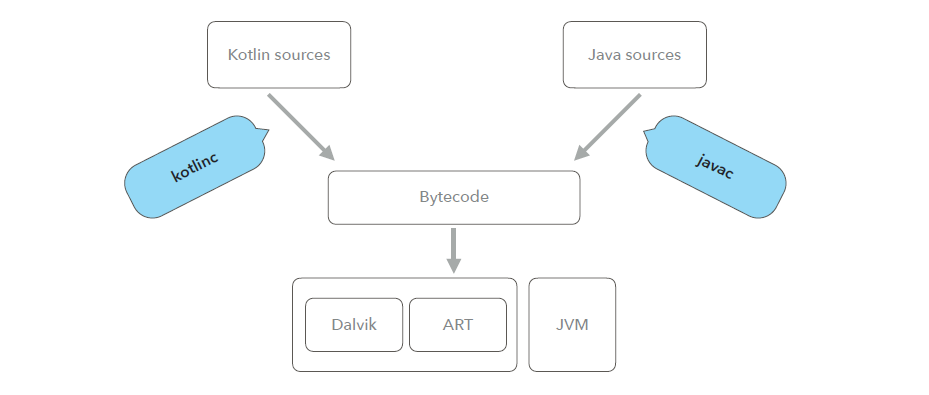
\includegraphics[scale=0.66]{KotlinCompiling.png}
  \caption{{\bfseries Schematizzazione del processo di compilazione}}
  \label{KotlinCompiling}
\end{figure}

\subsection{Conteggio dei metodi}
Questa problematica è spesso sottovalutata nella scelta dei linguaggi di programmazione da utilizzare, ma è molto importante, soprattutto in un ambito dalle risorse teoricamente limitate come quello dei sistemi mobile: quando 65.000 è il massimo dei metodi importabili in una applicazione, aggiungere una nuova libreria può risultare scoraggiante. Il cosiddetto problema del {\em method count} è stato, ad esempio, una discriminante nella scelta da parte di JetBrains di non utilizzare Scala come alternativa a Java (in quanto linguaggio che aggiunge un considerevole overhead in termini di method count), ma di sviluppare un nuovo linguaggio JVM. In generale è consigliato l'uso del tool {\bfseries ProGuard} \cite{proguard} per tagliare tutti i metodi non utilizzati; con questo tool, il method count di Kotlin su una generica applicazione Android risulta del 1.3\% \cite{ktProductionTales} rispetto al totale dei metodi presenti: pochissimi per un intero linguaggio.\\
Una discriminante in questo caso riguarda in particolare il modo in cui vengono implementate le lambda rispetto a Java 8, che è recentemente diventato disponibile in Android. In alcuni casi, Kotlin genera effettivamente un codice bytecode più efficiente attraverso l'uso di funzioni inline, il che significa che il codice è "allineato" alla linea di chiamata e il method count rimane così invariato. Di conseguenza, nel peggiore dei casi Kotlin, nello sviluppo di applicazioni Android, produce lo stesso numero di metodi di Java 8, nel caso migliore (e probabilmente medio) ancora più basso.\\

\subsection{Impatto sulle dimensioni e quantità di linee di codice}
Per quanto riguarda le dimensioni dei file apk generati da progetti scritti in Kotlin, si riscontra un leggero incremento: tipicamente, le applicazioni Kotlin risultano più pesanti di solo lo 0.6\% rispetto a quelle Java (anche qui utilizzando ProGuard). Diverso è il discorso riguardante le {\em lines-of-code}, infatti, come già discusso il linguaggio Kotlin porta una considerevole riduzione delle linee di codice: uno dei principi fondamentali della filosofia di Kotlin, infatti, è proprio la concisione, e questo si manifesta soprattutto scrivendo codice per Android. L'uso integrale di Kotlin all'interno della propria applicazione permette di ridurre, tipicamente, del 25\% il numero delle righe di codice impiegate per scriverla: un miglioramento decisamente notevole.\\

\subsection{Stabilità}
Un'altra preoccupazione manifestata dagli sviluppatori Java rispetto al passaggio al programmare in Kotlin è rappresentata dalla stabilità dell'applicazione. In questo caso, basta citare la filosofia Null-safety che Kotlin introduce: la produzione di crash da parte di un'applicazione dipende soprattutto dal programmatore, e in maniera decisamente minima dal linguaggio; tuttavia, Kotlin fornisce un sistema di tipi che previene in maniera sistematica gravi errori come le \texttt{NullPointerException} (che portano, appunto, al crash dell'applicativo), dunque aggiunge un ulteriore livello di stabilità rispetto a Java in questo senso.\\
